(by Vipin Singh)

\p
This chapter presents an analysis of the team structure essential for executing the business model.
It outlines the various roles within the organization and their contributions towards achieving the business objectives.
The focus lies on understanding the division of responsibilities and the collaborative efforts necessary for the company's growth and success.
This examination is intended to provide a clear view of the organizational framework and its significance in the operational realization of the business strategy.

\section{Team composition in the startup phase}
Since the business idea will start in a small scale, the human resources need to be used as efficiently as possible.
With only five founder members, this requires that each members role is not just defined by their job title.
Instead each member will have to be able to adapt and contribute across various facets of the business.
Still the business should also be able to scale up and expand its operations as it grows.

\p
With this said lets analyze the team composition, that is focused to rapidly develop and launch the product.

%TODO: Maybe create the table inline?
\begin{figure}[H]
    \centering
    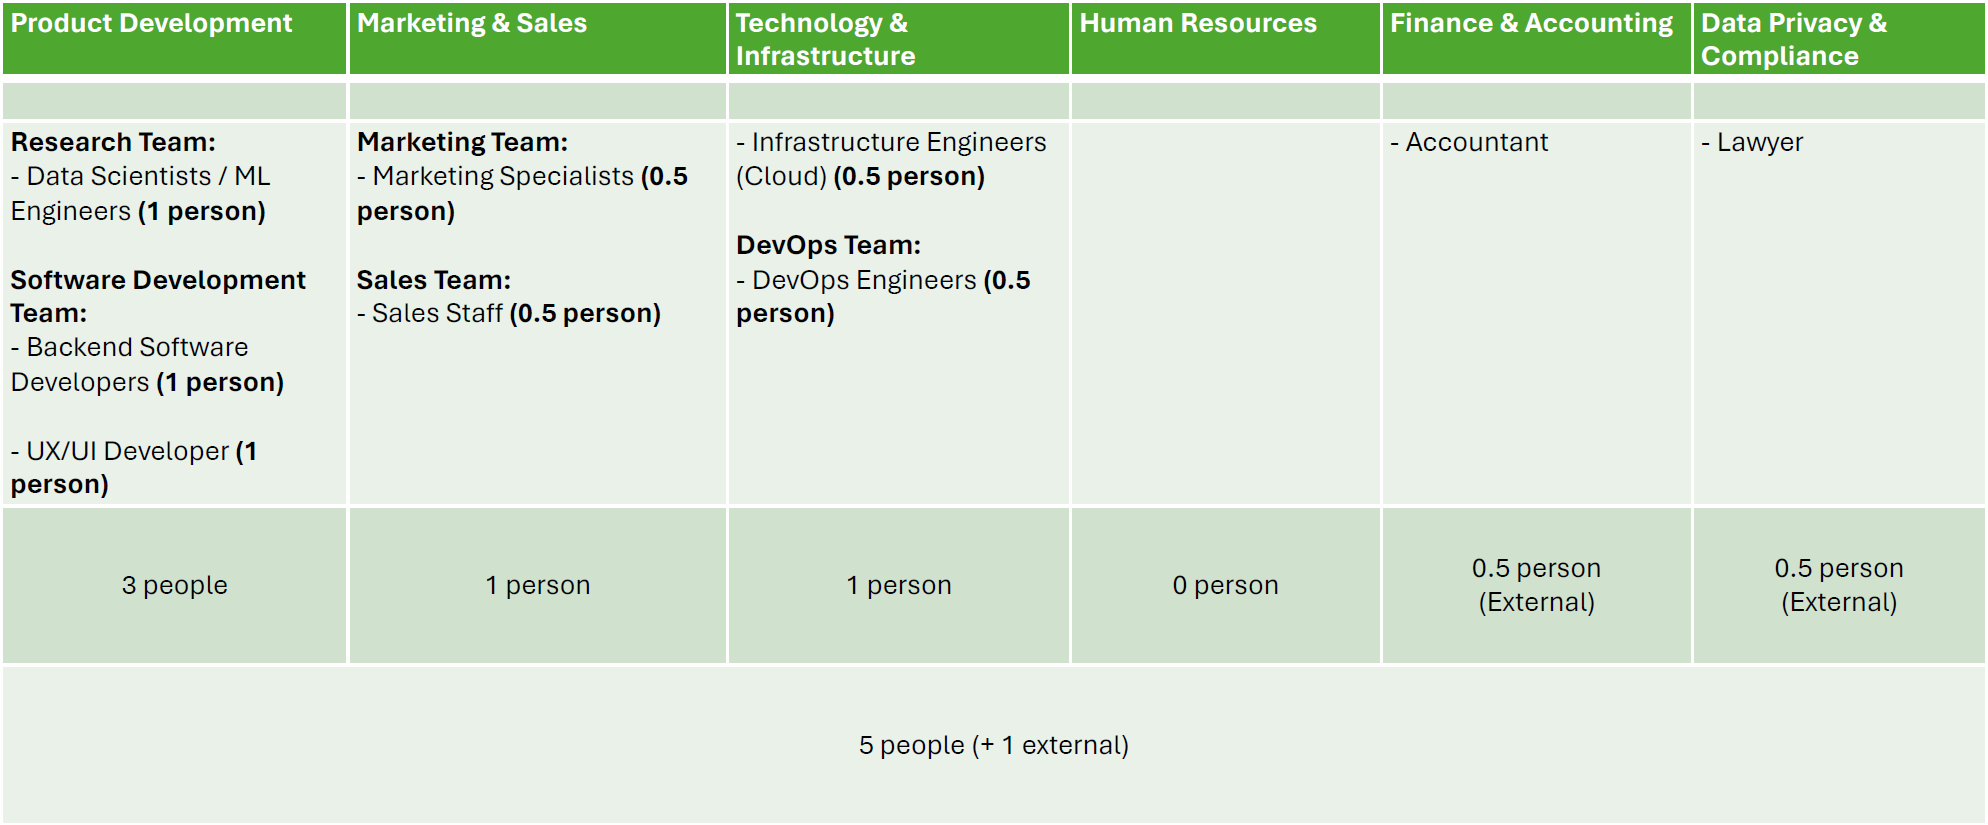
\includegraphics[width=\textwidth]{figures/team_comp_startup.png}
    \caption{Departments with team composition for a startup}
    \label{fig:team_comp_startup}
\end{figure}

In figure \ref{fig:team_comp_startup} we can see the team composition for a startup.
We decided to split the implementation of the team composition into six departments.
This department structure helps us to better understand the responsibilities we must fulfill for the business idea to succeed.
As we assign three out of the five founders to the product development department, it becomes clear that this is the core of our business for launching the product as fast as possible.

\p
Before we start with explaining the decisions for the team composition in figure \ref{fig:team_comp_startup}, we want to explain the responsibilities of each department and each role within the departments.
We will continue with the explanation of the decisions in subsection \ref{sub:decision_on_team_comp_startup}.

\subsection{Department: Product Development}
The \textbf{Product Development} department serves as the core of innovation in our company.
It is responsible for designing the product by converting research insights into practical features.
It also ensures that the product is developed such that it meets the markets demand and holds the technical superiority over its competitors.
It is split into two teams, the Research team and the Software Development team.

\subsubsection*{Research Team}
The research team guides the development of new product features by providing insights into the latest research in the field of ergonomics and posture detection.
Therefore they are mainly responsible for the machine learning pipeline.
\begin{itemize}
    \item \textbf{Data Scientists / ML Engineers:}
            \begin{itemize}
                \item Keep track of foundation models for the task
                \item Analyze data to improve prediction accuracy for the posture keypoints
                \item Finetune the foundation models for our specific tasks with collected data
                \item Collaborate with software developers to integrate the machine learning pipeline into the product
            \end{itemize}
\end{itemize}

\subsubsection*{Software Development Team}
The software development team directly implements the product features into the codebase.
They also ensure that the product is scalable and maintainable, while having the user experience in mind.
Another important task that is not mentioned directly in the following is the testing of the products features and the documentation of the codebase.
\begin{itemize}
    \item \textbf{Backend Software Developers:}
            \begin{itemize}
                \item Write and maintain the codebase
                \item Implement new features
                \item Ensure scalability
            \end{itemize}
    \item \textbf{UX/UI Developer:}
            \begin{itemize}
                \item Design the user interface
                \item Design prototypes for new features
                \item Implement the designs for the user interface into the codebase
            \end{itemize}
\end{itemize}

\subsection{Department: Marketing \& Sales}
The \textbf{Marketing \& Sales} department functions as a crucial link between the product and the potential customers.
Its primary responsibilities are the development of marketing strategies that communicate the value proposition of the product to the target audience.
Furthermore they drive the sales initiatives to convert prospects into customers.
This is critical to generate revenue for the company.
The alignment of marketing and sales efforts ensure the customer acquisition and retention, which is vital for growth and success.
For further structure this department is split into two teams, the Marketing team and the Sales team.

\subsubsection*{Marketing Team}
The marketing team is responsible for adjusting and exeecuting the marketing strategies and also monitoring the marketing trends.
\begin{itemize}
    \item \textbf{Marketing Specialists:}
            \begin{itemize}
                \item Execute marketing campaigns
                \item Analyze campaign performance
                \item Manage content creation
                \item Design marketing media (e.g. flyers, posters, etc.)
                \item Ensure brand consistency
            \end{itemize}
\end{itemize}

\subsubsection*{Sales Team}
The sales team is responsible for the customer relationships and to identify potential customer segments.
Additionally they are togeether with the marketing team responsible to reach out to high potential customer segments.
\begin{itemize}
    \item \textbf{Sales Staff:}
            \begin{itemize}
                \item Reach out to potential clients
                \item Conduct sales pitches
                \item Negotiate contracts with B2B customers and close deals
            \end{itemize}
\end{itemize}

\subsection{Department: Technology \& Infrastructure}
The \textbf{Technology \& Infrastructure} serves as the foundational support for the company's internal operations.
This department ensures that the product is built on a reliable and advanced technological base.
Additionally they guarantee for uninterrupted service delivery and scalability internally but also for the customers.
The dual focus is crucial for the future growth of the company, allowing it to adapt to an evolving technological landscape.
They also setup systems for the company's employeees to work efficiently in projects.
\begin{itemize}
    \item \textbf{IT Support Staff:}
            \begin{itemize}
                \item Technical support to employees
                \item Perform maintenance and update on company hardware and software infrastructure
            \end{itemize}
    \item \textbf{DevOps Engineers:}
            \begin{itemize}
                \item Develop and maintain CI/CD (Continuous Integration/Continuous Development) pipelines
                \item Collaborate with software developers on code releases and deployments
                \item Implement automation tools to reduce manual processes
                \item Implement physical and network infrastructure to operate services
                \item Optimize the compute infrastructure and data storage
                \item Devlop and implement network security policies and procedures against unauthorized access
            \end{itemize}
\end{itemize}

\subsection{Department: Human Resources}
The \textbf{Human Resources} department plays a vital role in shaping the organization's talent and culture.
This department focuses primarily on recruiting skilled individuals who can contribute to the company's growth.
Additionally, the department is responsible for implementing training programs to enhance the employees' skills and knowledge.
They are also taking care of the administrative tasks, such as the employees' time registration and their holidays.

\subsection{Department: Finance \& Accounting}
The \textbf{Finance \& Accounting} department is there to maintain the financial integrity of the company.
Its primary responsibilities involve the comprehensive management of the company's finances.
This includes tasks such as budgeting (efficient allocation of resources), financial reporting (transparency of fiscal health), and accounting (accuracy and reliability of financial documentation).
Additionally, the department is tasked with overseeing the financial compliance, such as adherence to the tax regulations.
Furthermore, the department plays a role in optimizing financial planning and execution.
This is an essential prerequisite for the long-term growth and success of the company.

\begin{itemize}
    \item \textbf{Accountant:}
    \begin{itemize}
        \item Manage transactions and financial records
        \item Create invoices for the B2B customers according to the negotiations of the sales team
        \item Prepare tax returns and payments
        \item Maintain compliance with tax regulations
    \end{itemize}
\end{itemize}

\subsection{Department: Data Privacy \& Compliance}
The \textbf{Data Privacy \& Compliance} department is essential for ensuring the company's adherence to data protection laws and industry regulations.
Their primary tasks include maintaining compliance across the company's operations and preparing for the implementation of ISO certification guidelines.
This department plays a key role in upholding data ethics and legal conformity, crucial for the company's integrity and trustworthiness.

\begin{itemize}
    \item \textbf{Lawyer:}
            \begin{itemize}
                \item Ensure compliance with relevant laws and regulations
                \item Review business contracts and provide support in disputes
            \end{itemize}
\end{itemize}

\subsection{Decisions on the team composition for the startup phase}
\label{sub:decision_on_team_comp_startup}

In this subsection we want to explain the decisions we made for the team composition in figure \ref{fig:team_comp_startup}.
As already mentioned, since the main goal of the startup phase is to launch the product as fast as possible, we decided to assign three out of the five founders to the Product Development department.
The roles that are assigned in the product development department are the following:
\begin{itemize}
    \item Data Scientist / ML Engineer \textbf{(1 person)}
    \item Backend Software Developer \textbf{(1 person)}
    \item UX/UI Developer \textbf{(1 person)}
\end{itemize}
With these we have covered the most important roles in order to develop the first prototypes and develop these further to a product that can be launched.

These three members will need to work closely together and engage in a broader scope of tasks beyond just their dedicated roles to effectively develop the product in a small team.

\p
The remaining two founders are assigned to the Marketing \& Sales department and the Technology \& Infrastructure department.
Lets first look at the Marketing \& Sales department:
\begin{itemize}
    \item Marketing Specialist \textbf{(0.5 person)}
    \item Sales Staff \textbf{(0.5 person)}
\end{itemize}
Be aware that we assign only one person to the Marketing \& Sales department because we assume that one person working as both Marketing Specialist and Sales Staff is enough for the startup phase.
We also considered that the person working in this department will closely work together members of the Product Development department, especially with the UX/UI Developer.
They can together create marketing strategies to promote the product with the first prototypes and also create marketing media, such as flyers and posters.

\p
As mentioned the last founder is assigned to the Technology \& Infrastructure department:
\begin{itemize}
    \item Infrastructure Engineer \textbf{(0.5 person)}
    \item DevOps Engineer \textbf{(0.5 person)}
\end{itemize}
Similar to the Marketing \& Sales department we assign only one person to the Technology \& Infrastructure department because we assume that one person working as both Infrastructure Engineer and DevOps Engineer is enough for the startup phase.
The member working in this department will work closely together with the Backend Software Developer to setup the infrastructure for the product.

\p
The remaining departments, Human Resources, Finance \& Accounting and Data Privacy \& Compliance, are not assigned to any of the founders.
For the case of the Human Resources department we assume that the founders will take care of the administrative tasks, such as time registration and their holidays.
In that case there is no need for any employee in the Human Resources department.

\p
For the remaining two departments we seek to outsource the tasks to external companies.
For the Finance \& Accounting department we will outsource the tasks to an external accounting company, that will take care of the financial integrity of the company.
For the Data Privacy \& Compliance department we will outsource the tasks to an external lawyer, that will help us to ensure the company's adherence to data protection laws and industry regulations.

\p
With this we have covered all the departments and the roles within the departments for the startup phase.
We should be able to launch the product with this team composition of the five founder members.
After the product is launched we can start to scale up the company and hire more employees.
This leads to the next section \ref{sec:team_comp_highscaled}, where we will analyze the team composition after the company has scaled up.

\section{Team composition after higher scaling}
\label{sec:team_comp_highscaled}

\begin{figure}[H]
    \centering
    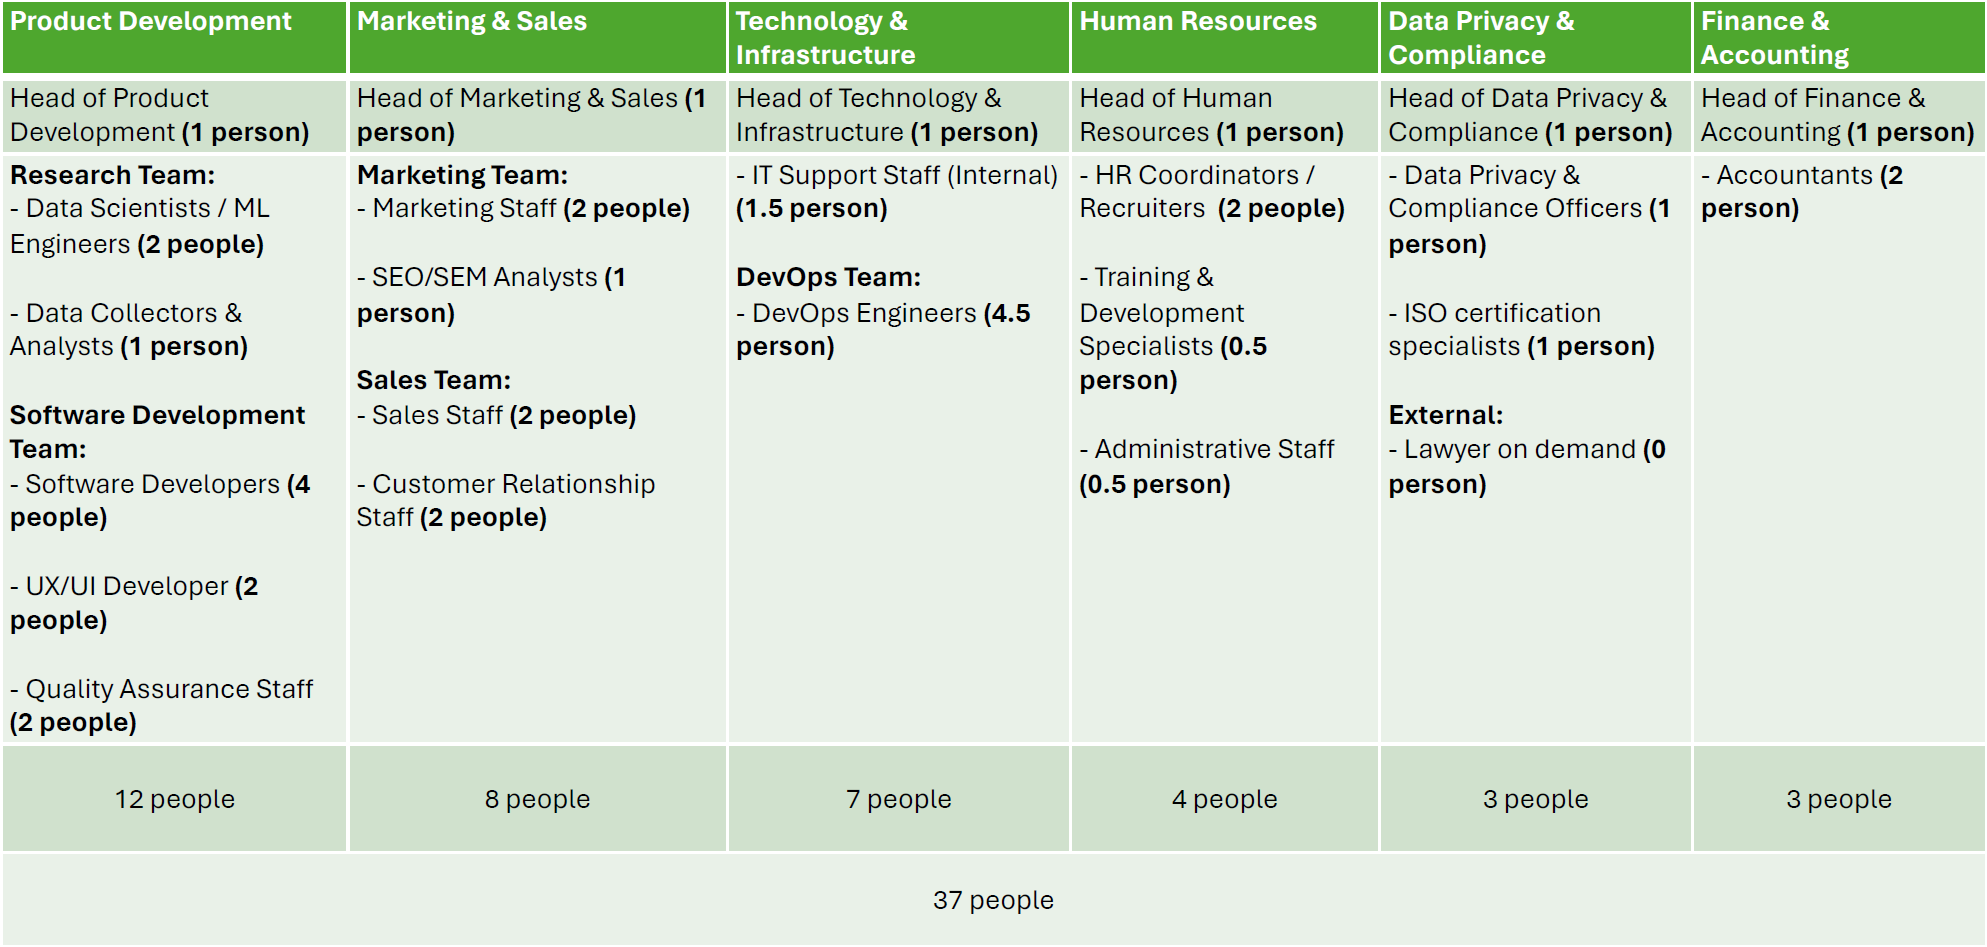
\includegraphics[width=\textwidth]{figures/team_comp_highscaled.png}
    \caption{Departments with team composition after the company has scaled up}
    \label{fig:team_comp_highscaled}
\end{figure}